% ============================================================
%  J3 — MATIN : Autograd — Rétropropagation depuis Zéro
%  Julien Rolland — M2 Développement Fullstack
% ============================================================
\documentclass[aspectratio=169, 10pt]{beamer}
% ============================================================
%  PREAMBLE COMMUN — IA, Deep Learning & Machine Learning
%  Julien Rolland — M2 Développement Fullstack
% ============================================================

% --- Langue & encodage ---
\usepackage[utf8]{inputenc}
\usepackage[T1]{fontenc}
\usepackage{babel}
\babelprovide[import, main]{french}

% --- Thème Beamer ---
\usetheme{Madrid}
\usecolortheme{default}

% Palette de bleu académique
\definecolor{jedy_blue}{RGB}{0, 51, 102}       % bleu foncé principal
\definecolor{jedy_mid}{RGB}{0, 102, 179}        % bleu moyen accent
\definecolor{jedy_light}{RGB}{204, 221, 240}    % bleu très clair (fond boxes)
\definecolor{jedy_alert}{RGB}{180, 30, 30}      % rouge pour alertes
\definecolor{jedy_example}{RGB}{0, 120, 60}     % vert pour exemples

% Application des couleurs sur le thème Madrid
\setbeamercolor{palette primary}{bg=jedy_blue, fg=white}
\setbeamercolor{palette secondary}{bg=jedy_mid, fg=white}
\setbeamercolor{palette tertiary}{bg=jedy_blue, fg=white}
\setbeamercolor{palette quaternary}{bg=jedy_blue, fg=white}
\setbeamercolor{structure}{fg=jedy_blue}
\setbeamercolor{frametitle}{bg=jedy_blue, fg=white}
\setbeamercolor{title}{bg=jedy_blue, fg=white}
\setbeamercolor{block title}{bg=jedy_mid, fg=white}
\setbeamercolor{block body}{bg=jedy_light, fg=black}
\setbeamercolor{block title alerted}{bg=jedy_alert, fg=white}
\setbeamercolor{block body alerted}{bg=jedy_light, fg=black}
\setbeamercolor{block title example}{bg=jedy_example, fg=white}
\setbeamercolor{block body example}{bg=jedy_light, fg=black}

% --- Typographie ---
\usepackage{lmodern}
\setbeamerfont{title}{size=\Large, series=\bfseries}
\setbeamerfont{frametitle}{size=\normalsize, series=\bfseries}

% --- Navigation : suppression des icônes de navigation par défaut ---
\setbeamertemplate{navigation symbols}{}

% --- Numérotation des slides ---
\setbeamertemplate{footline}{%
  \leavevmode%
  \hbox{%
    \begin{beamercolorbox}[wd=.333\paperwidth,ht=2.25ex,dp=1ex,center]{author in head/foot}%
      \usebeamerfont{author in head/foot}\insertshortauthor
    \end{beamercolorbox}%
    \begin{beamercolorbox}[wd=.334\paperwidth,ht=2.25ex,dp=1ex,center]{title in head/foot}%
      \usebeamerfont{title in head/foot}\insertshorttitle
    \end{beamercolorbox}%
    \begin{beamercolorbox}[wd=.333\paperwidth,ht=2.25ex,dp=1ex,right]{date in head/foot}%
      \usebeamerfont{date in head/foot}
      \insertframenumber{} / \inserttotalframenumber\hspace*{2ex}
    \end{beamercolorbox}%
  }%
  \vskip0pt%
}

% --- Maths ---
\usepackage{amsmath, amssymb, amsthm}
\usepackage{bm}          % vecteurs en gras : \bm{w}

% --- Code source ---
\usepackage{listings}
\usepackage{xcolor}

\lstdefinestyle{pythonstyle}{
  language=Python,
  basicstyle=\ttfamily\footnotesize,
  keywordstyle=\color{jedy_blue}\bfseries,
  commentstyle=\color{gray}\itshape,
  stringstyle=\color{jedy_example},
  numberstyle=\tiny\color{gray},
  numbers=left,
  numbersep=5pt,
  frame=single,
  framerule=0.4pt,
  rulecolor=\color{jedy_light},
  backgroundcolor=\color{jedy_light!40},
  breaklines=true,
  showstringspaces=false,
  tabsize=4,
}
\lstset{style=pythonstyle}

% Alias pratique pour code inline
\newcommand{\code}[1]{\texttt{\small#1}}

% --- Graphiques ---
\usepackage{graphicx}
\usepackage{tikz}
\usetikzlibrary{arrows.meta, positioning, shapes.geometric, fit, calc}
\usepackage{pgfplots}
\pgfplotsset{compat=1.18}

% --- Tableaux ---
\usepackage{booktabs}
\usepackage{array}

% --- Icônes (optionnel, nécessite fontawesome5) ---
% \usepackage{fontawesome5}

% --- Macros ML/DL courantes ---
\newcommand{\R}{\mathbb{R}}
\newcommand{\E}{\mathbb{E}}
\newcommand{\Loss}{\mathcal{L}}
\newcommand{\dataset}{\mathcal{D}}
\newcommand{\X}{\mathbf{X}}
\newcommand{\y}{\mathbf{y}}
\newcommand{\w}{\mathbf{w}}
\newcommand{\W}{\mathbf{W}}
\newcommand{\grad}{\nabla}
\newcommand{\T}{^{\top}}         % transposée : \X\T
\newcommand{\lr}{\alpha}         % learning rate
\newcommand{\norm}[1]{\left\|#1\right\|}

% Encadré "Objectif pédagogique" en début de section
\newenvironment{objectif}{%
  \begin{alertblock}{Objectif}%
}{%
  \end{alertblock}%
}

% --- Infos du cours (remplacer dans chaque slides.tex) ---
\author[J. Rolland]{Julien Rolland}
\institute[Jedy]{Formation M2 Développement Fullstack}


\title[Autograd]{Autograd --- Rétropropagation depuis Zéro}
\subtitle{Jour 3 --- Matin}
\date{Jour 3}

% ============================================================
\begin{document}
% ============================================================

\begin{frame}
  \titlepage
\end{frame}

\begin{frame}{Plan du module}
  \tableofcontents
\end{frame}

% ============================================================
\section{Limite du Linéaire}
% ============================================================

\begin{frame}{La Limite du Linéaire : Le Problème du XOR}
  \begin{columns}[T]
    \begin{column}{0.46\textwidth}
      \begin{block}{Rappel J2 : Un neurone = une droite}
        \begin{itemize}
          \item $y = \text{sign}(\bm{w} \cdot \bm{x} + b)$
          \item Sépare l'espace en deux \textbf{demi-plans}
        \end{itemize}
      \end{block}
      \smallskip
      \begin{alertblock}{XOR : Non linéairement séparable}
        \begin{itemize}
          \item Classe {\color{jedy_blue}$\bullet$} : $(0,0)$ et $(1,1)$
          \item Classe {\color{jedy_alert}$\blacktriangle$} : $(0,1)$ et $(1,0)$
          \item \textbf{Aucune droite} ne les sépare
        \end{itemize}
      \end{alertblock}
      \smallskip
      \begin{exampleblock}{Solution}
        «~Tordre l'espace~» $\Rightarrow$ \textbf{Couches cachées} (\textit{Hidden Layers})
      \end{exampleblock}
    \end{column}
    \begin{column}{0.50\textwidth}
      \centering
      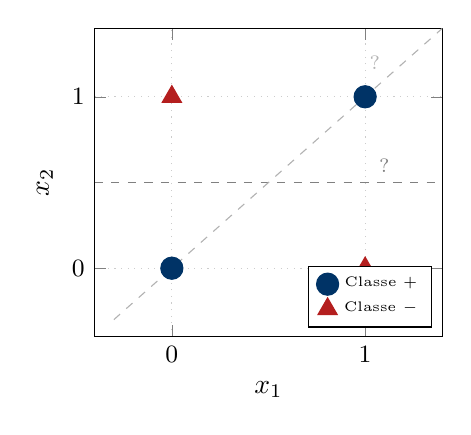
\begin{tikzpicture}
        \begin{axis}[
          width=6cm, height=5.5cm,
          xmin=-0.4, xmax=1.4,
          ymin=-0.4, ymax=1.4,
          xtick={0,1}, ytick={0,1},
          xlabel={$x_1$}, ylabel={$x_2$},
          xlabel style={font=\small},
          ylabel style={font=\small},
          tick label style={font=\small},
          axis lines=box,
          grid=major,
          grid style={dotted, gray!40},
          legend pos=south east,
          legend style={font=\tiny, fill=white},
        ]
          \addplot[only marks, mark=*, mark size=4pt, color=jedy_blue]
            coordinates {(0,0) (1,1)};
          \addlegendentry{Classe $+$}
          \addplot[only marks, mark=triangle*, mark size=4pt, color=jedy_alert]
            coordinates {(0,1) (1,0)};
          \addlegendentry{Classe $-$}
          \addplot[dashed, gray, domain=-0.4:1.4, samples=2, forget plot] {0.5};
          \addplot[dashed, gray!60, domain=-0.3:1.4, samples=2, forget plot] {x};
          \node[gray, font=\scriptsize] at (axis cs:1.1, 0.6) {?};
          \node[gray!60, font=\scriptsize] at (axis cs:1.05, 1.2) {?};
        \end{axis}
      \end{tikzpicture}
    \end{column}
  \end{columns}
\end{frame}

% ============================================================
\section{La Non-Linéarité}
% ============================================================

\begin{frame}{L'Ingrédient Secret : La Non-Linéarité}
  \begin{columns}[T]
    \begin{column}{0.42\textwidth}
      \begin{alertblock}{Sans activation : réseau inutile}
        \small
        \[W_2(W_1 \cdot \X) = \underbrace{(W_2 W_1)}_{W_{\text{comb}}} \cdot \X\]
        1000 couches = 1 seule couche linéaire
      \end{alertblock}
      \smallskip
      \begin{exampleblock}{Avec activation $\sigma$ : expressivité}
        \small
        $h = \sigma(W_1 \cdot \X)$ puis $y = W_2 h$\\
        $\Rightarrow$ \textbf{Non réductible} à une seule couche
      \end{exampleblock}
      \smallskip
      \begin{block}{ReLU : La Norme Industrielle}
        \small
        $f(x) = \max(0, x)$ \quad Dérivée : $0$ ou $1$
      \end{block}
    \end{column}
    \begin{column}{0.55\textwidth}
      \centering
      \begin{tikzpicture}
        \begin{groupplot}[
          group style={
            group size=1 by 2,
            vertical sep=0.7cm,
          },
          width=6cm, height=2.5cm,
          axis lines=center,
          xtick={-2,0,2},
          xticklabel style={font=\tiny},
          yticklabel style={font=\tiny},
          domain=-3:3,
          samples=80,
          xmin=-3, xmax=3,
          clip=false,
        ]
          \nextgroupplot[
            ymin=-0.3, ymax=3.2,
            ytick={0,1,2,3},
            title={\small\bfseries ReLU : $f(x) = \max(0,x)$},
          ]
          \addplot[jedy_blue, very thick] {max(0,x)};

          \nextgroupplot[
            ymin=-0.1, ymax=1.2,
            ytick={0,0.5,1},
            title={\small\bfseries Sigmoïde : $\sigma(x) = \frac{1}{1+e^{-x}}$},
          ]
          \addplot[jedy_alert, very thick] {1/(1+exp(-x))};
        \end{groupplot}
      \end{tikzpicture}
    \end{column}
  \end{columns}
\end{frame}

% ============================================================
\section{Credit Assignment}
% ============================================================

\begin{frame}{Le «~Credit Assignment Problem~»}
  \begin{columns}[T]
    \begin{column}{0.50\textwidth}
      \begin{block}{Dans un réseau profond}
        \begin{itemize}
          \item On calcule $\Loss$ à la \textbf{sortie}
          \item Les poids $w_1, w_2, \ldots$ sont au \textbf{début}
          \item \textbf{Question :} de combien modifier $w_i$ pour réduire $\Loss$ ?
        \end{itemize}
      \end{block}
      \smallskip
      \begin{alertblock}{Le problème fondamental}
        L'influence d'un poids précoce passe par \textbf{toutes les couches suivantes}
      \end{alertblock}
      \smallskip
      \begin{exampleblock}{Solution : Rétropropagation}
        Propager $\frac{\partial \Loss}{\partial w_i}$ \textbf{à l'envers} le long du graphe
      \end{exampleblock}
    \end{column}
    \begin{column}{0.46\textwidth}
      \centering
      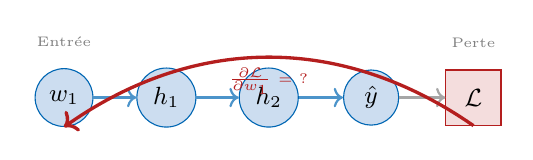
\begin{tikzpicture}[
        node distance=1.3cm,
        neuron/.style={circle, draw=jedy_mid, fill=jedy_light,
                       minimum size=0.7cm, font=\small\bfseries},
        loss/.style={rectangle, draw=jedy_alert, fill=jedy_alert!15,
                     minimum size=0.7cm, font=\small\bfseries},
        lbl/.style={font=\tiny, color=gray},
      ]
        \node[neuron] (w1)  {$w_1$};
        \node[neuron, right of=w1]  (h1)  {$h_1$};
        \node[neuron, right of=h1]  (h2)  {$h_2$};
        \node[neuron, right of=h2]  (out) {$\hat{y}$};
        \node[loss,   right of=out] (L)   {$\Loss$};

        \draw[->, thick, jedy_mid!70] (w1) -- (h1);
        \draw[->, thick, jedy_mid!70] (h1) -- (h2);
        \draw[->, thick, jedy_mid!70] (h2) -- (out);
        \draw[->, thick, gray!70]     (out) -- (L);

        \draw[->, very thick, jedy_alert, bend right=35]
          (L.south) to
          node[below, midway, font=\tiny, color=jedy_alert]
            {$\frac{\partial\Loss}{\partial w_1}$ = ?}
          (w1.south);

        \node[lbl, above=0.15cm of w1] {Entrée};
        \node[lbl, above=0.15cm of L]  {Perte};
      \end{tikzpicture}
    \end{column}
  \end{columns}
\end{frame}

% ============================================================
\section{Graphe de Calcul}
% ============================================================

\begin{frame}{Le Graphe de Calcul (DAG)}
  \begin{columns}[T]
    \begin{column}{0.44\textwidth}
      \begin{block}{Modélisation}
        \begin{itemize}
          \item Toute fonction $\Rightarrow$ graphe \textbf{orienté acyclique}
          \item \textbf{Nœuds} : opérations élémentaires ($+$, $\times$, $\exp$\ldots)
          \item \textbf{Arêtes} : variables / tenseurs
        \end{itemize}
      \end{block}
      \vspace{1pt}
      \begin{exampleblock}{Intérêt}
        Chaque nœud calcule sa \textbf{dérivée locale} $\Rightarrow$ les gradients se chaînent vers l'entrée
      \end{exampleblock}
      \vspace{1pt}
      \begin{block}{Notre exemple}
        $f(x, y) = (x + y) \times y$\\[0.2em]
        \quad$a = x + y$,\quad $b = a \times y$
      \end{block}
    \end{column}
    \begin{column}{0.52\textwidth}
      \centering
      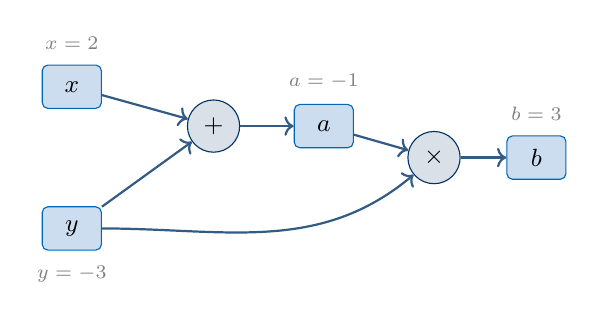
\begin{tikzpicture}[
        var/.style={rectangle, draw=jedy_mid, fill=jedy_light, rounded corners=2pt,
                    minimum width=0.75cm, minimum height=0.55cm, font=\small\bfseries},
        op/.style={circle, draw=jedy_blue, fill=jedy_blue!15,
                   minimum size=0.65cm, font=\small\bfseries},
        arr/.style={->, thick, color=jedy_blue!80},
        val/.style={font=\scriptsize, color=gray},
      ]
        \node[var] (x)    at (0,   0.9)  {$x$};
        \node[var] (y)    at (0,  -0.9)  {$y$};
        \node[op]  (plus) at (1.8, 0.4)  {$+$};
        \node[var] (a)    at (3.2, 0.4)  {$a$};
        \node[op]  (mul)  at (4.6, 0)    {$\times$};
        \node[var] (b)    at (5.9, 0)    {$b$};

        \draw[arr] (x) -- (plus);
        \draw[arr] (y) -- (plus);
        \draw[arr] (y) to[out=0, in=220] (mul);
        \draw[arr] (plus) -- (a);
        \draw[arr] (a) -- (mul);
        \draw[arr] (mul) -- (b);

        \node[val, above] at (0,   1.25)  {$x=2$};
        \node[val, below] at (0,  -1.25)  {$y=-3$};
        \node[val, above] at (3.2, 0.75)  {$a=-1$};
        \node[val, above] at (5.9, 0.35)  {$b=3$};
      \end{tikzpicture}
    \end{column}
  \end{columns}
\end{frame}

% ============================================================
\section{Forward \& Backward Pass}
% ============================================================

\begin{frame}[fragile]{Le Forward Pass}
  \begin{columns}[T]
    \begin{column}{0.40\textwidth}
      \begin{block}{Mécanique}
        \begin{enumerate}
          \item Parcourir le graphe de \textbf{gauche à droite}
          \item Calculer chaque nœud
          \item \textbf{Stocker} les valeurs intermédiaires
        \end{enumerate}
      \end{block}
      \smallskip
      \begin{alertblock}{Pourquoi stocker ?}
        Les valeurs intermédiaires sont \textbf{nécessaires} lors du backward pass pour calculer les dérivées locales
      \end{alertblock}
    \end{column}
    \begin{column}{0.56\textwidth}
      \begin{lstlisting}[style=pythonstyle]
x = 2.0
y = -3.0

# Noeud 1 : addition
a = x + y   # a = -1.0

# Noeud 2 : multiplication
b = a * y   # b = 3.0  <- Sortie

print(f"Sortie b = {b}")
# Sortie b = 3.0
      \end{lstlisting}
    \end{column}
  \end{columns}
\end{frame}

\begin{frame}{La Chain Rule (Règle de la Chaîne)}
  \begin{columns}[T]
    \begin{column}{0.46\textwidth}
      \begin{block}{Formule}
        Si $z = f(y)$ et $y = g(x)$, alors :
        \[\frac{\partial z}{\partial x} = \frac{\partial z}{\partial y} \cdot \frac{\partial y}{\partial x}\]
      \end{block}
      \smallskip
      \begin{exampleblock}{Pour les graphes de calcul}
        \begin{itemize}
          \item \textbf{Gradient amont} $\frac{\partial \Loss}{\partial y}$ arrive de la sortie
          \item Nœud calcule sa \textbf{dérivée locale} $\frac{\partial y}{\partial x}$
          \item \textbf{Gradient aval} = amont $\times$ local
        \end{itemize}
      \end{exampleblock}
    \end{column}
    \begin{column}{0.50\textwidth}
      \centering
      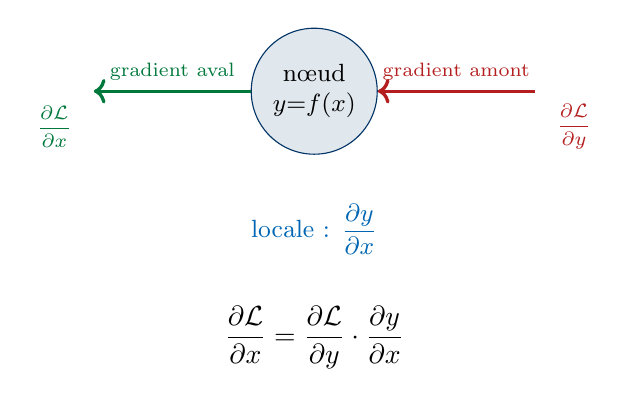
\begin{tikzpicture}[
        op/.style={circle, draw=jedy_blue, fill=jedy_blue!12,
                   minimum size=1.6cm, align=center, font=\small},
      ]
        \node[op] (node) at (0, 0) {nœud\\$y{=}f(x)$};

        \draw[->, very thick, jedy_alert]
          (2.8, 0) -- (node)
          node[midway, above, font=\scriptsize, color=jedy_alert]
            {gradient amont};
        \node[color=jedy_alert, font=\scriptsize] at (3.3, -0.45)
          {$\dfrac{\partial \Loss}{\partial y}$};

        \draw[->, very thick, jedy_example]
          (node) -- (-2.8, 0)
          node[midway, above, font=\scriptsize, color=jedy_example]
            {gradient aval};
        \node[color=jedy_example, font=\scriptsize] at (-3.3, -0.45)
          {$\dfrac{\partial \Loss}{\partial x}$};

        \node[font=\small, color=jedy_mid, below=0.5cm of node]
          {locale : $\dfrac{\partial y}{\partial x}$};

        \node[font=\normalsize, below=1.8cm of node]
          {$\dfrac{\partial \Loss}{\partial x} = \dfrac{\partial \Loss}{\partial y} \cdot \dfrac{\partial y}{\partial x}$};
      \end{tikzpicture}
    \end{column}
  \end{columns}
\end{frame}

\begin{frame}[fragile]{Le Backward Pass (Reverse Mode)}
  \begin{columns}[T]
    \begin{column}{0.38\textwidth}
      \begin{block}{Algorithme}
        \begin{enumerate}
          \item Initialiser $\frac{\partial \Loss}{\partial \Loss} = 1$
          \item Parcourir \textbf{de droite à gauche}
          \item Chaque nœud : grad aval $\times$ dérivée locale
        \end{enumerate}
      \end{block}
      \smallskip
      \begin{exampleblock}{Résultat clé}
        \textbf{Un seul backward}\\
        $\Rightarrow$ gradients de \textbf{tous} les paramètres
      \end{exampleblock}
    \end{column}
    \begin{column}{0.58\textwidth}
      \begin{lstlisting}[style=pythonstyle]
# b = a * y  =>  db/da = y,  db/dy = a
# a = x + y  =>  da/dx = 1,  da/dy = 1

# Init : gradient de la sortie
db = 1.0

# Noeud * : b = a * y
da   = db * y    # 1.0 * (-3.0) = -3.0
dy_2 = db * a    # 1.0 * (-1.0) = -1.0

# Noeud + : a = x + y
dx   = da * 1.0  # -3.0
dy_1 = da * 1.0  # -3.0

# Gradients finaux (accumulation)
grad_x = dx            # -3.0
grad_y = dy_2 + dy_1   # -4.0
      \end{lstlisting}
    \end{column}
  \end{columns}
\end{frame}

% ============================================================
\section{Micro-Autograd en Python}
% ============================================================

\begin{frame}[fragile]{Software Design : La Classe \texttt{Value}}
  \begin{columns}[T]
    \begin{column}{0.34\textwidth}
      \begin{block}{Encapsuler le \texttt{float}}
        \begin{itemize}\small
          \item \code{data} : valeur numérique
          \item \code{grad} : gradient (init. à 0)
          \item \code{\_prev} : parents dans le graphe
          \item \code{\_backward} : gradient local
        \end{itemize}
      \end{block}
      \smallskip
      \begin{exampleblock}{Principe}
        Code mathématique \textbf{normal} + construction du graphe \textbf{automatique}
      \end{exampleblock}
    \end{column}
    \begin{column}{0.62\textwidth}
      \begin{lstlisting}[style=pythonstyle]
class Value:
    def __init__(self, data, _children=()):
        self.data = data
        self.grad = 0.0
        self._prev = set(_children)
        self._backward = lambda: None

    def __repr__(self):
        return (f"Value(data={self.data:.3f}, "
                f"grad={self.grad:.3f})")

# Utilisation
x = Value(2.0)
y = Value(-3.0)
print(x)  # Value(data=2.000, grad=0.000)
      \end{lstlisting}
    \end{column}
  \end{columns}
\end{frame}

\begin{frame}[fragile]{Magie Python : Operator Overloading}
  \begin{columns}[T]
    \begin{column}{0.34\textwidth}
      \begin{block}{Dunder methods}
        \begin{itemize}\small
          \item \code{\_\_add\_\_} $\rightarrow$ opérateur $+$
          \item \code{\_\_mul\_\_} $\rightarrow$ opérateur $\times$
          \item Graphe construit \textbf{implicitement}
        \end{itemize}
      \end{block}
      \smallskip
      \begin{alertblock}{Règle pour $+$}
        \small
        $\dfrac{\partial(a+b)}{\partial a} = 1$,\quad $\dfrac{\partial(a+b)}{\partial b} = 1$
      \end{alertblock}
      \smallskip
      \begin{alertblock}{Règle pour $\times$}
        \small
        $\dfrac{\partial(a \cdot b)}{\partial a} = b$,\quad $\dfrac{\partial(a \cdot b)}{\partial b} = a$
      \end{alertblock}
    \end{column}
    \begin{column}{0.62\textwidth}
      \begin{lstlisting}[style=pythonstyle]
def __add__(self, other):
    out = Value(self.data + other.data,
                (self, other))
    def _backward():
        self.grad  += 1.0 * out.grad
        other.grad += 1.0 * out.grad
    out._backward = _backward
    return out

def __mul__(self, other):
    out = Value(self.data * other.data,
                (self, other))
    def _backward():
        self.grad  += other.data * out.grad
        other.grad += self.data  * out.grad
    out._backward = _backward
    return out
      \end{lstlisting}
    \end{column}
  \end{columns}
\end{frame}

% ============================================================
\section{Vers PyTorch}
% ============================================================

\begin{frame}{De Scalaires vers les Tenseurs}
  \begin{columns}[T]
    \begin{column}{0.50\textwidth}
      \begin{block}{Ce matin : Micro-Autograd scalaire}
        \begin{itemize}
          \item Autograd sur des \textbf{scalaires} ($x \in \R$)
          \item Graphe construit manuellement
          \item Gradients : nombres simples
        \end{itemize}
      \end{block}
      \smallskip
      \begin{exampleblock}{PyTorch : Même logique, Tenseurs}
        \begin{itemize}
          \item Variables : \textbf{tenseurs} $X \in \R^{m \times n}$
          \item Graphe construit \textbf{automatiquement}
          \item Gradients : matrices (Jacobiennes)
        \end{itemize}
      \end{exampleblock}
    \end{column}
    \begin{column}{0.46\textwidth}
      \begin{center}
        \renewcommand{\arraystretch}{1.4}
        \begin{tabular}{lll}
          \toprule
          & \textbf{Scalaire} & \textbf{Tenseur} \\
          \midrule
          Valeur   & $x \in \R$        & $X \in \R^{m \times n}$ \\
          Gradient & $\partial\Loss/\partial x$ & $\partial\Loss/\partial X$ \\
          Type     & scalaire          & Jacobienne \\
          Règle    & Chaîne            & Chaîne vectorielle \\
          Classe   & \code{Value}      & \code{torch.Tensor} \\
          \bottomrule
        \end{tabular}
      \end{center}
      \smallskip
      \begin{alertblock}{Cet après-midi : PyTorch}
        \small\code{x = torch.tensor(..., requires\_grad=True)}
      \end{alertblock}
    \end{column}
  \end{columns}
\end{frame}

\end{document}
